\Chapter{Simulations}  \label{simulations}
%%%%%%%%%%%%%%%%%%%%%%%%%%%%%%%%%%%%%%%%%%%%%%%%%%%%%%%%%%%%%%%%%%%%%%%%%%%%%%%%
%%%%%%%%%%%%%%%%%%%%%%%%%%%%%%%%%%%%%%%%%%%%%%%%%%%%%%%%%%%%%%%%%%%%%%%%%%%%%%%%
\Section{Introduction}\label{sec:code}
%%%%%%%%%%%%%%%%%%%%%%%%%%%%%%%%%%%%%%%%%%%%%%%%%%%%%%%%%%%%%%%%%%%%%%%%%%%%%%%%
%%%%%%%%%%%%%%%%%%%%%%%%%%%%%%%%%%%%%%%%%%%%%%%%%%%%%%%%%%%%%%%%%%%%%%%%%%%%%%%%

With the rapid improvement in computing resources and codes in recent years,  
accelerator facilities can now strive to rely on accurate beam dynamics simulations. 
These simulations model single particle effects 
(e.g. particle tracking in a magnetic field) as well as collective effects such as space charge (SC),  
and coherent synchrotron radiation (CSR).
Accurate simulations can benefit accelerator communities in several ways.
Before beam line construction countless configurations can be tested in simulation.
This can prevent costly hardware mistakes. 
Predictive power with respect to beam dynamics could also significantly reduce the amount of time 
spent configuring the machine for various experiments. This is key for the AWA
where the operating charge is changed often, and so the optics must change as well.

The beam dynamics reported in this thesis, were simulated with 
the open source, particle-in-cell (PIC) code \verb|OPAL| \cite{opal}. 
PIC codes simulate the electromagnetic forces that particles see in an accelerator. 
This is done by mapping the input particles onto a grid. 
Then in each time (or z) step, the forces due to space charge, accelerating gradients, 
and magnets are calculated and applied to the grid.
\verb|OPAL| comes in two flavors, \verb|OPAL-cycl| and \verb|OPAL-t|. The first is used to model 
cyclotrons, and the latter, which is used for this work, is suited for photoinjectors. 
\verb|OPAL-t| was chosen in part because it models the 3D space charge necessary to accurately simulate the high charge bunches at the AWA. 
It was chosen for several reasons:
\begin{itemize}
	\item Ability to calculate transverse space charge and wakefield forces 
	\item Option to run the code in parallel
	\item Data recorded in global and local reference frames 
	\item Free and open source (freely available to the public)
\end{itemize} 

The first item is crucial to standard operations at the AWA. Especially in the 
case of TBA, a high charge is needed in the drive beam line, therefore transverse 
space charge forces must be calculated in the simulations to give realistic results.
Typical charge for a TBA experiment at the AWA is \SI{40}{nC}. 
This is much higher than other facilities that usually operate at \SI{1}{nC} or below. 
Higher charge also means higher emittances, which can reach \SI{100}{\micro\meter}, 
if beam transport is not optimized.

The ability to run the code in parallel dramatically reduced the amount of simulation time needed. 
For example, simulating the gun and linac, about \SI{15}{m} of elements,
with 100,000 particles on one core would take about 30 minutes. 
When the number of cores is increased to 16, the same run takes less than 
5 minutes. This reduction in time by ~80\%, combined with the capability to run 
many cases at once on the cluster allows for more efficient use of time.
Typical running conditions were simulated on 16 cores, random samples used up to 128 cores, 
and up to 5,200 cores were used for large optimization runs.
\lsnote{\it I have no idea what you meant by `random samples'.}

The accelerator model used for the simulations in this chapter is the AWA drive line operated at \SI{40}{nC}. 
This beam line consists of a gun, solenoids, six linac cavities, and quadrupoles.
This is the line that will be used to feed high charge bunch trains to the PETS, 
which will be installed downstream. Optimization of this beam line was done at \SI{40}{nC}
to improve beam line settings during future experiments.
A model-based method was used for the initial simulations presented in this chapter. The results showed that 
it is best to run the RF cavities off crest to compensate for energy spread in the gun. 
The model-based method was compared to a genetic algorithm (GA) as a verification test.
The results from both methods were similar, and the GA method was used for beam line design work in Chapter~\ref{chp:4}.

%%%%%%%%%%%%%%%%%%%%%%%%%%%%%%%%%%%%%%%%%%%%%%%%%%%%%%%%%%%%%%%%%%%%%%%%%%%%%%%%
%%%%%%%%%%%%%%%%%%%%%%%%%%%%%%%%%%%%%%%%%%%%%%%%%%%%%%%%%%%%%%%%%%%%%%%%%%%%%%%%
\Section{Benchmarking}\label{sec:bench}

Initially \verb|OPAL-t| was benchmarked against commonly used particle tracking codes \verb|ASTRA| and \verb|GPT|.  
This ensured correct use of the code, and reliability of \verb|OPAL-t|.  
Two collective effects of particular interest to the AWA were included in the investigation: 
space charge (SC) and coherent synchrotron radiation (CSR).
The beam dynamics of a \SI{1}{nC} drive beam in the photoinjector were used as 
the model for comparison in the space charge study. 
A $20^{\circ}$ hard edge dipole magnet was used to benchmark CSR effects in 
\verb|GPT| and \verb|OPAL-t| by bending a \SI{1}{nC} beam 
at energies between \SI{2}{Mev} and \SI{100}{MeV}.  
The results of these benchmark studies are presented below, 
including a discussion of the similarities and differences between the codes.
 
The AWA group has used several beam codes in the past including:\\
\mbox{T-STEP/PARMELA}~\cite{parmela}, \verb|ASTRA|~\cite{astra}, and \verb|GPT|~\cite{gpt}.  
In order to take advantage of computing resources offered by 
Argonne National Laboratory (ANL), an investigation of 
\verb|OPAL|~\cite{opal} was done; this is an open source and parallel code that comes in two flavors;  
\verb|OPAL-cycl| and \verb|OPAL-t|. The latter was installed on the Blues and Bebop high performance computing clusters
at the Laboratory Computing Resource Center (LCRC) provided by ANL~\cite{lcrc}.
(See Appendix~\ref{build} for instruction on how to build \verb|OPAL-t| at ANL.)

\Subsection{Gun Simulations}
The SC algorithms were probed using the AWA photoinjector, 
an RF gun which is a 1.5-cell copper standing-wave cavity at \SI{1.3}{GHz}, 
with bucking, focusing, and matching solenoids. 
In the remainder of this thesis, the word gun is used 
in place of photoinjector. The simulation parameters were chosen to 
approximately generate the canonical ``2D transverse emittance of
\SI{1}{\micro\metre} at bunch charge \SI{1}{nC}'' case.  
The initial beam parameters were based on gun operations at PITZ \cite{pitz},
due to the similarities between the PITZ and AWA RF guns.
The PITZ parameters came close to achieving the \SI{1}{\micro\metre}
target without any optimization. A coarse 1D minimization
using the golden section method~\cite{golden} of the 
emittance was done to determine the value of the laser radius 
used in this benchmark. The resulting minimum emittance was   
\SI{1.16}{\micro\metre}. 

The initial bunch distribution parameters as well as the 
on-axis gun gradient, and magnetic field of the solenoids used in 
the benchmark are listed in Table~\ref{tab:bench}. 
The RF gun and solenoid field maps were generated 
with the SUPERFISH/POISSON  codes~\cite{superfish}.
The gradient was chosen to match typical operations at PITZ~\cite{pitz}
and the AWA. The RF and solenoid fields seen by the beam in the gun are shown in Figure~\ref{fig:gunfields}.
\begin{table}
	\begin{center}
		\caption{Input simulation parameters for gun benchmark.}
		\label{tab:bench}
		\begin{tabular}{l l} 
	\toprule
	\toprule
	\textbf{Parameter} & \textbf{Value} \\ 
	\midrule
	Charge  & \SI{1}{nC} \\
	Gradient & \SI{60}{MV/m} \\
	
	Phase & Max energy (on crest) \\
	
	Laser radius & \SI{0.75}{mm} \\
	
	Rise and fall time & \SI{6}{ps} \\
	
	Initial kinetic energy & \SI{0.55}{eV} \\
	
	Matching solenoid strength & \SI{-0.389}{T} \\
	
	Buck and focusing solenoid strength & \SI{-0.12}{T} \\
	\bottomrule			
\end{tabular}
	\end{center}
\end{table}
\begin{figure}
	\begin{center}
		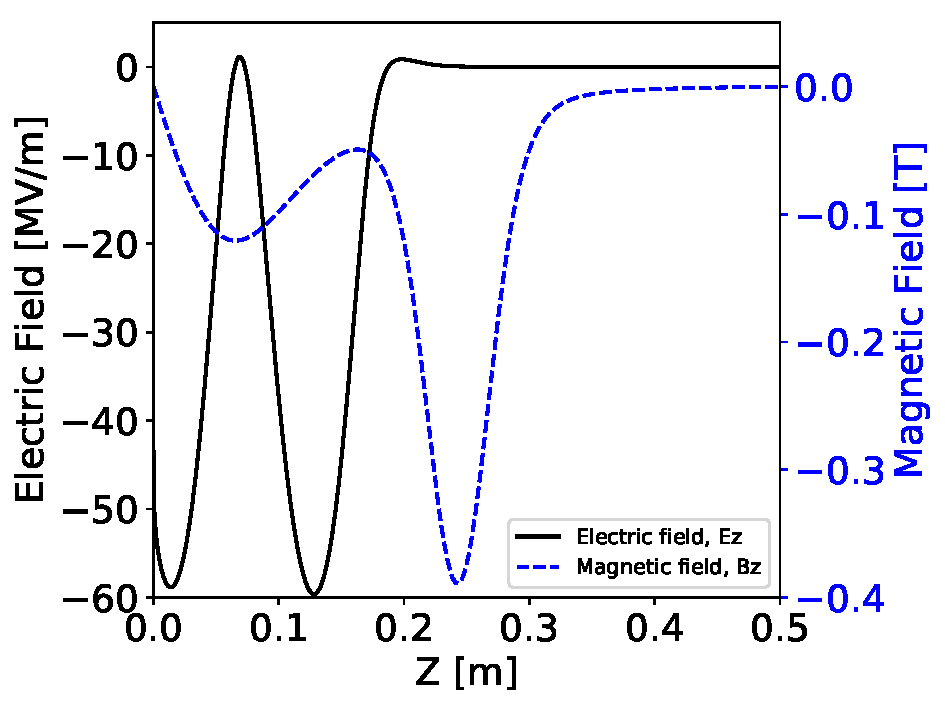
\includegraphics[width=0.75\textwidth]{images/gun_EM_fields}
		\caption{Electric and magnetic fields seen by the beam on axis in the gun. 
			The gun ends at \SI{0.3}{m}. }
		\label{fig:gunfields}
	\end{center}
\end{figure}

Note that the codes use various methods to model 
the RF and magnetic fields, SC, and image charge. 
The \verb|ASTRA| simulations used the axial E field of the  
gun and solenoids, and then extended the fields to find the
transverse components using the paraxial approximation 
(e.g. $E_r=-\frac{r}{2}\frac{dE_z}{dz}$). 
The simulation used a 2D cylindrical-symmetric SC algorithm with a uniform  
particle-deposition mesh; see \verb|ASTRA| user manual~\cite{astra}.
The radial and longitudinal number of cells composing the mesh 
were $N_r=32$ and $N_z=64$, with 100k particles.  
The image charge close to the cathode was accounted for until 
the bunch reached \SI{9.7}{cm} from the cathode surface. 

\verb|GPT| read in the 2D electric and magnetic field files,  
and used a square 3D adaptive SC mesh with $N_x=N_y=N_z=46$
with 100,000 particles, see spacecharge3Dmesh option in \verb|GPT| manual~\cite{gpt}.
To calculate image charge, \verb|GPT| uses a Dirichlet boundary condition at the  
cathode ($z=0$). The calculation is turned off when the  
distance between the beam and cathode is longer than the 
mesh box. \verb|OPAL-t| also read in the field maps, and used a block 
structured equidistant SC mesh, see \verb|OPAL| manual for SC calculation~\cite{opal}.  
Several square mesh sizes were run in \verb|OPAL-t|. The results plotted in 
Figure~\ref{fig:benchplot_gun} and~\ref{fig:benchplot_5m} 
correspond to a mesh of $N_x=N_y=N_z=46$, with 1 million particles. 
The image charge calculation uses a 
shifted integrated Green function \cite{imagecharge}.  
\begin{figure}
	\begin{center}
		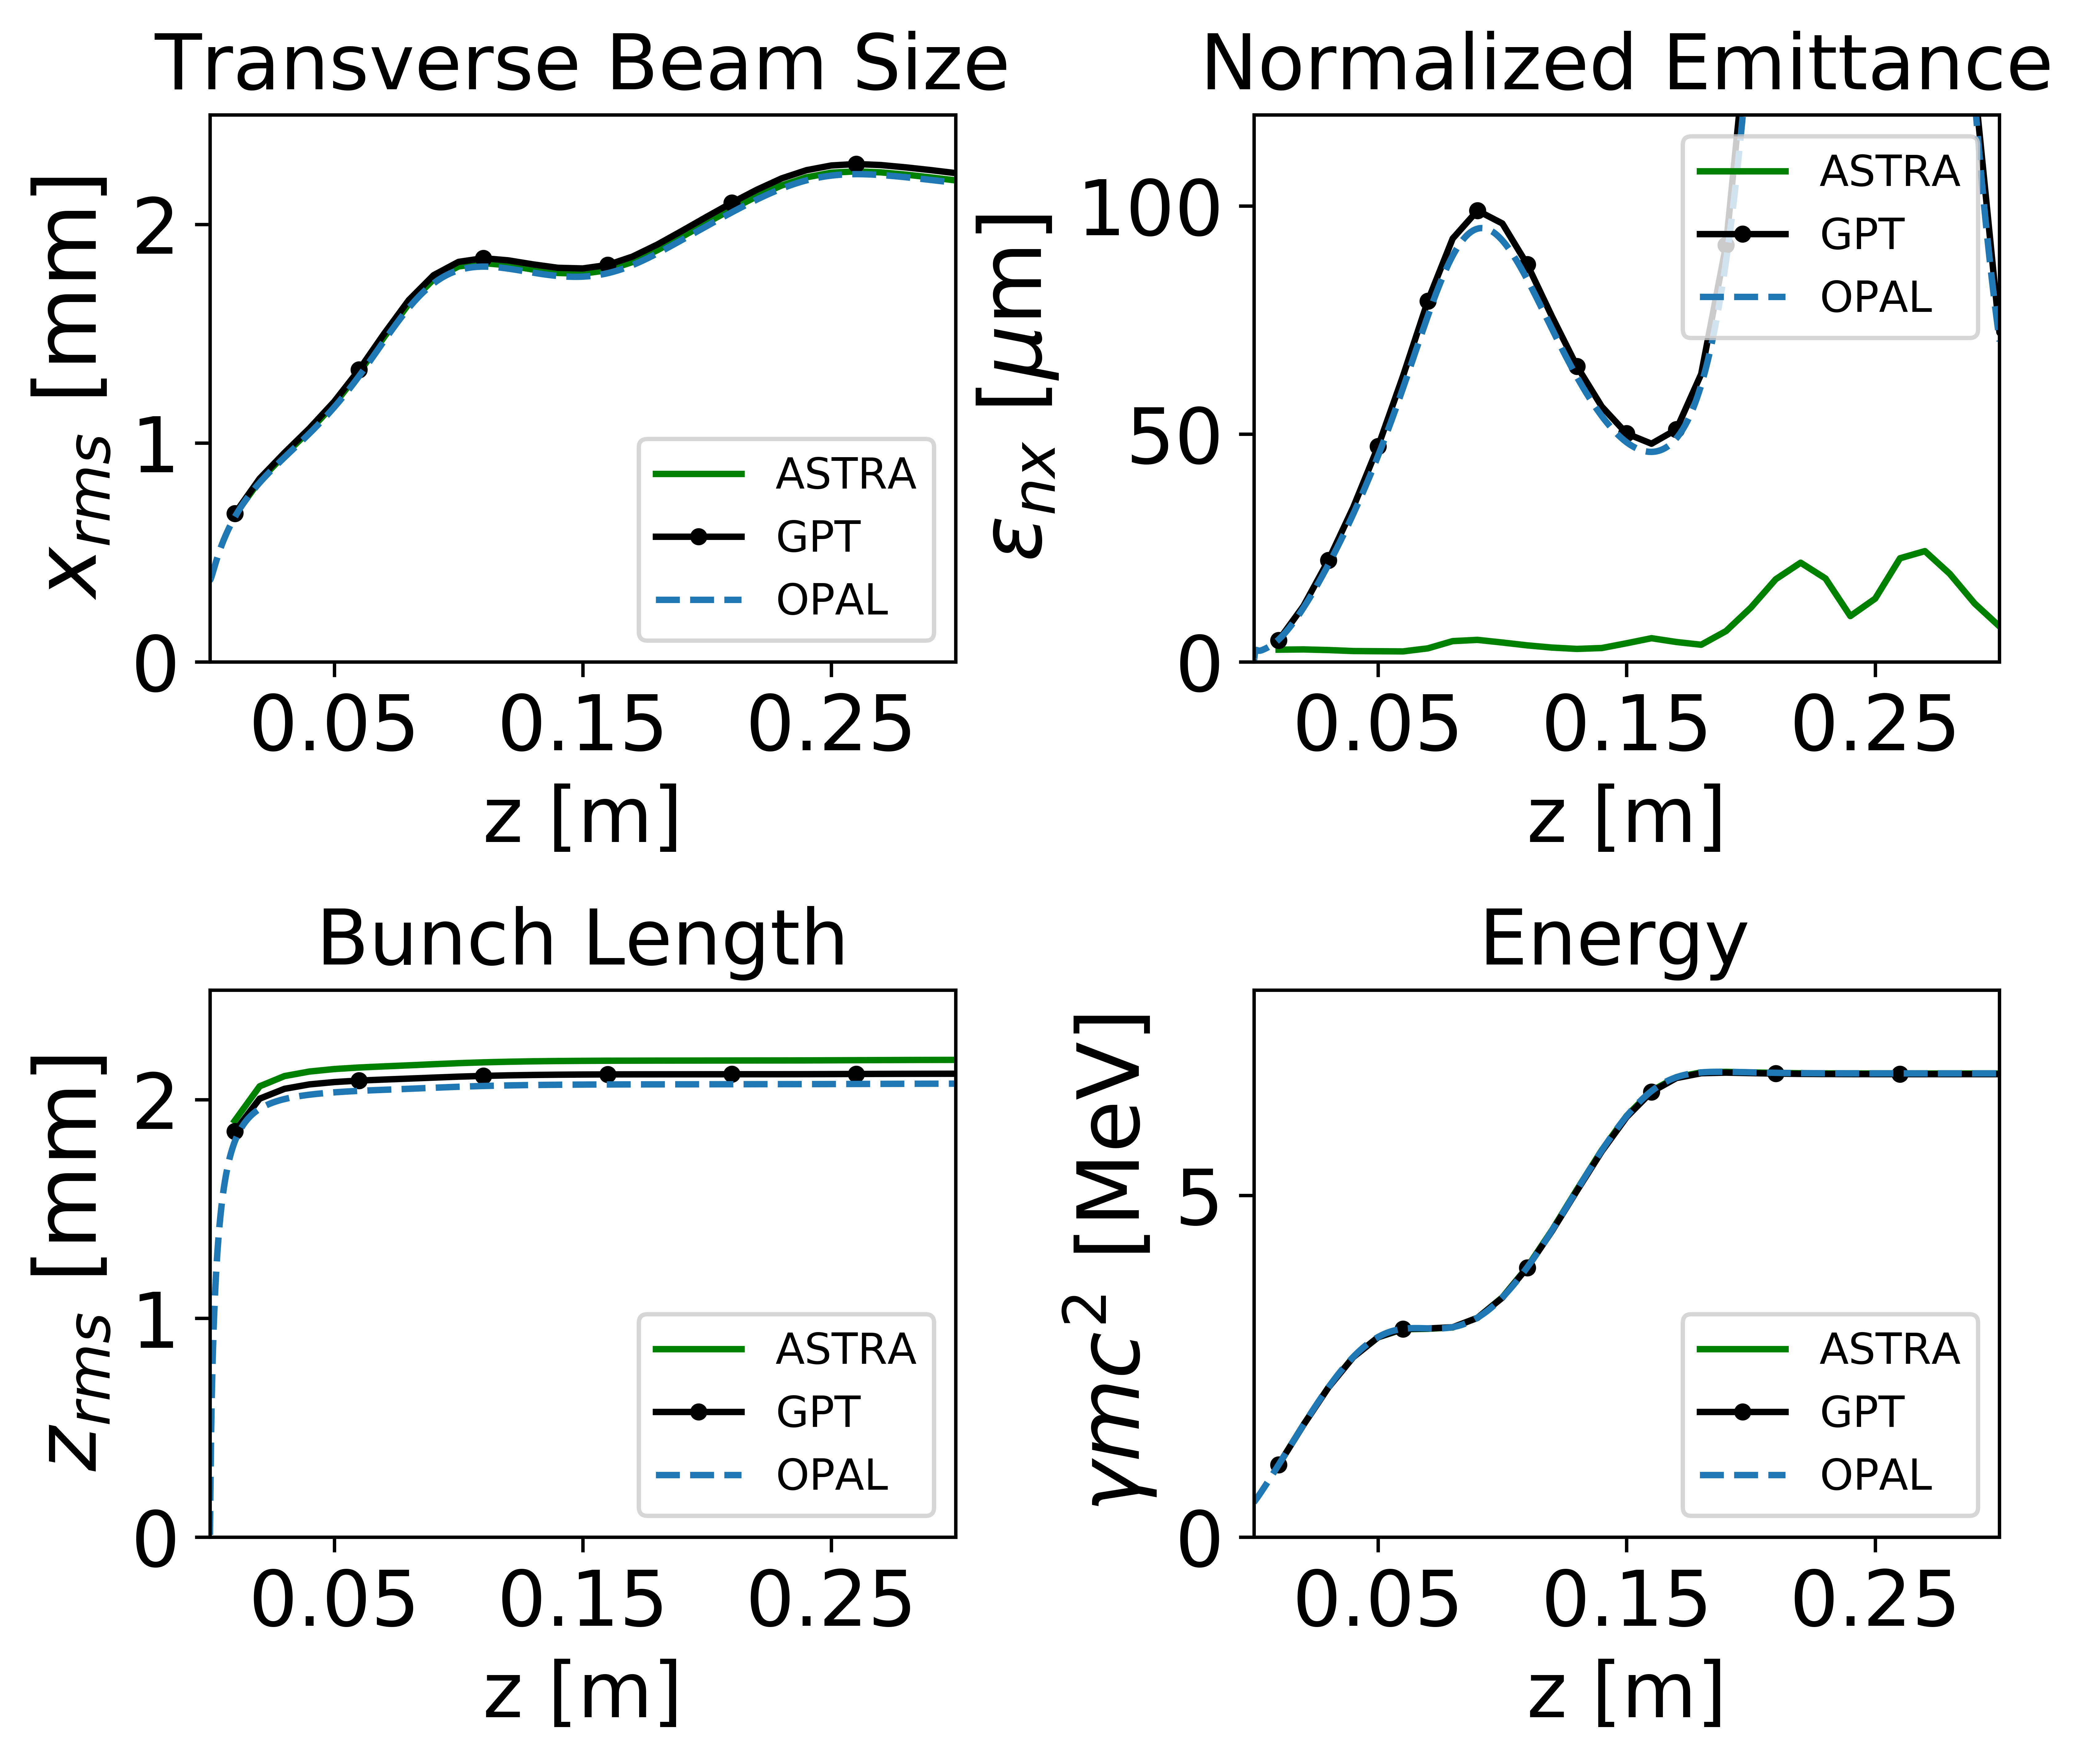
\includegraphics[width=0.8\textwidth]{images/benchmark_gun}
		\caption{Beam envelopes in the gun for benchmark between \verb|OPAL|, \verb|ASTRA|, and \verb|GPT|.}
	    \label{fig:benchplot_gun}

        \vspace*{\floatsep}
        
		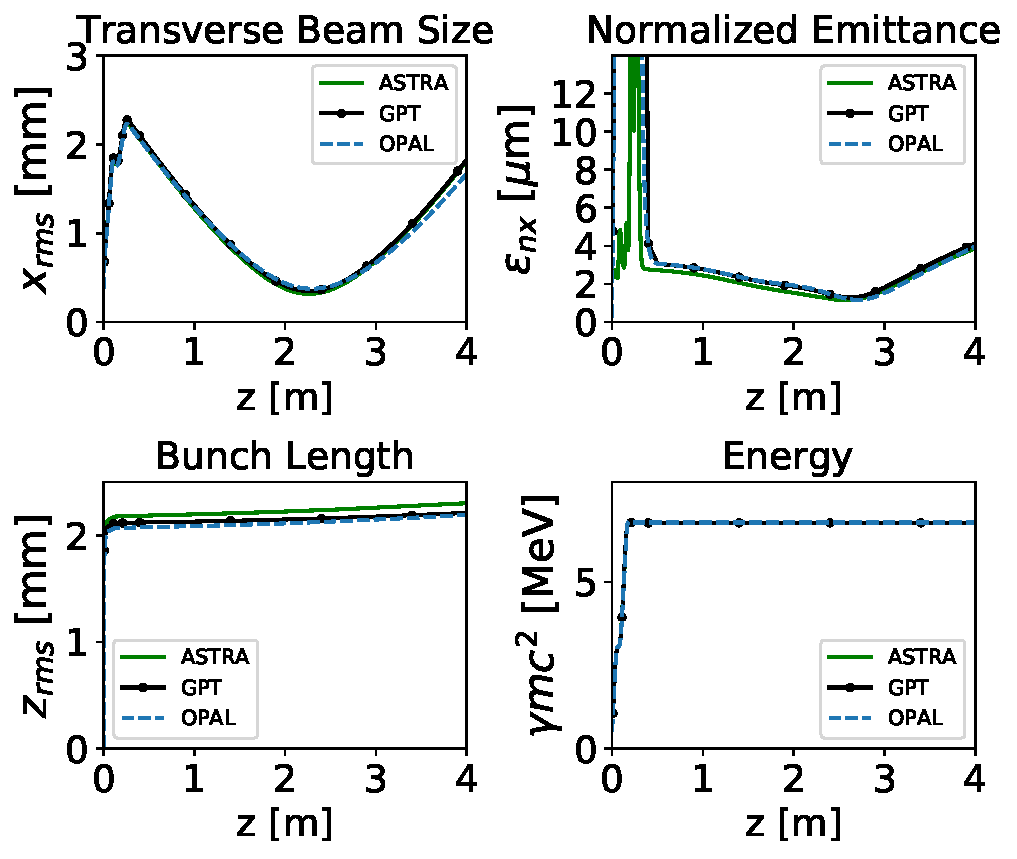
\includegraphics[width=0.8\textwidth]{images/benchmark_5m}
		\caption{Beam envelopes in drift for benchmark between \verb|OPAL|, \verb|ASTRA|, and \verb|GPT|.}
	    \label{fig:benchplot_5m}
	\end{center}
\end{figure}

In general, the simulation results are in reasonable agreement 
and within expectations based on previous benchmarks \cite{codecompare}. 
See Figure~\ref{fig:benchplot_gun} and~\ref{fig:benchplot_5m} 
for a comparison of the beam envelopes generated by the three simulations in the gun and drift. 
The apparent disagreement of emittance between \verb|ASTRA| and the other
two codes in the gun is because the former removes the angular momentum   
induced by the solenoid, while the other two codes do not. 
After the beam exits the solenoid, the emittance results  
are in good agreement, as shown in Figure~\ref{fig:benchplot_5m}.

\Subsection{Dipole Simulations}
Simulations of a hard edge dipole were done in \verb|GPT|  
and \verb|OPAL-t| in order to probe the CSR results.
Short mono-energetic bunches with a Gaussian energy distribution with zero initial transverse emittance  
were sent through the dipole.  Beam and dipole parameters are shown in Table~\ref{tab:benchcsr}. 
The CSR routine used in \verb|OPAL-t| is based on the routine used in ELEGANT \cite{elegant}, 
which is known to assume the beam is ultra-relativistic. The CSR routine in \verb|GPT|  
does not use the ultra-relativistic approximation ($\beta=1$) 
and as a result, works at all energies \cite{gptcsr}.  
Therefore, the routines were expected to match well at high energy and  
diverge at lower energy. Results of the CSR simulations are shown in Figure~\ref{fig:csr}  
As expected, the results between \verb|GPT| and \verb|OPAL-t| disagree at low energies. 
\begin{table}
	\begin{center}
		\caption{Input simulation parameters for CSR benchmark.}
		\label{tab:benchcsr}
		\begin{tabular}{l l} 
			\toprule
			\toprule
			\textbf{Parameter} & \textbf{Value} \\ 
			\midrule
			Dipole Length & \SI{0.3}{m} \\
			$\sigma_x =\sigma_y$ & \SI{1}{mm} \\
			$\sigma_z$ 			 & \SI{0.3}{mm} \\
			Bend Angle 			 & \SI{20}{^\circ} \\
			Energy (Mono-energetic)	 & \SI{2}{MeV} to \SI{100}{MeV} \\
			\bottomrule			
		\end{tabular}
	\end{center}
\end{table}
\begin{figure}
	\centering
	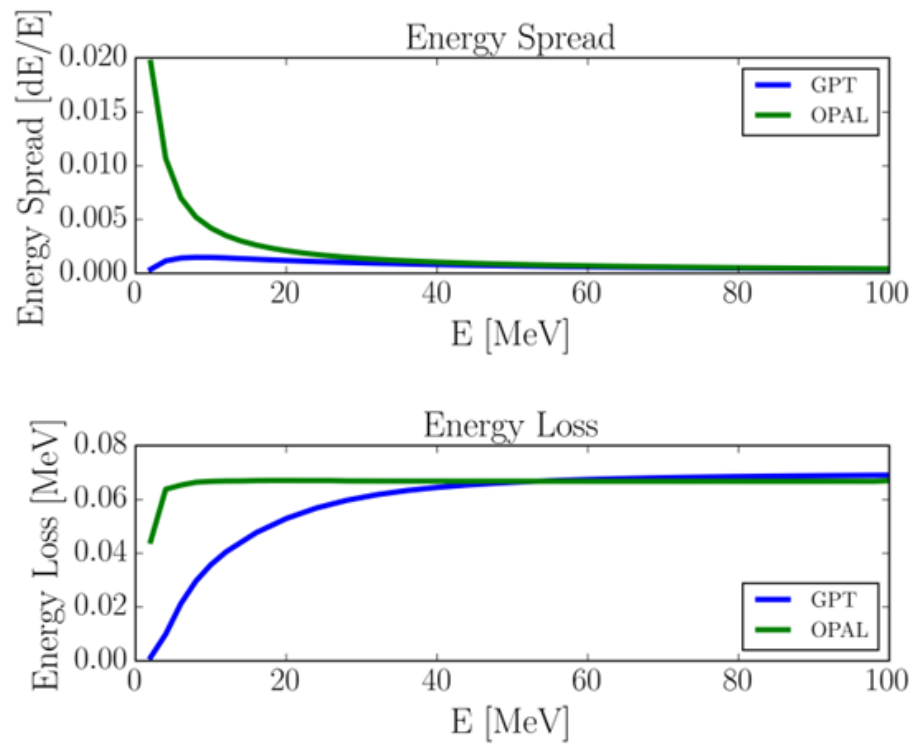
\includegraphics[width=0.5\textwidth]{./images/CSR}
	\caption{Results of CSR benchmark between \verb|OPAL| and \verb|GPT|.
	The codes agree well at high energies and diverge, as expected, at low energies.}
	\label{fig:csr}
\end{figure}

\Subsection{Benchmark Conclusion}
In summary, all three codes (\verb|OPAL|, \verb|ASTRA|, \verb|GPT|), agreed well when modeling a photoinjector
with space charge effects, solenoid and RF fields.
\verb|OPAL| and \verb|GPT| also agree on energy loss and energy spread calculations at high energy.
At low energy they diverge, and \verb|GPT| is more accurate because it calculates 
$\beta$ at all times instead of assuming the beam is relativistic.
Preference on which code to use depends more on ease of use 
and availability, especially for the AWA facility where $\beta\approx 1$. 

\Section{Convergence Studies}

The \verb|OPAL| code was chosen for modeling of the AWA after benchmarking was complete.
Convergence runs were done for three parameters: 
time step, SC mesh size, and number of particles.  
Each case was tested in the gun using the same field maps and 
baseline settings that were used to compare SC in \verb|OPAL-t|,  
\verb|ASTRA|, and \verb|GPT| in Section~\ref{sec:bench}. 
All \verb|OPAL-t| simulations were run on 
sixteen cores, taking advantage of parallel calculations. 
The number of particles was varied from 20,000 to 3.2 million.  
The longitudinal parameters (energy,  bunch length)  
showed no variation, but there were slight deviations 
in the transverse emittance and beam size. The same results 
were observed when the time step was varied from \SI{0.1}{ps} to \SI{10}{ps}.  
When the grid size was changed from 32, 44, 46, and $64^3$ ; 
again the results lacked any major discrepancies.  
In all cases, no appreciable differences were observed in the energy,
emittance, beam size, or bunch length. In  most  cases,  
if unreasonable  parameters  were chosen, 
\verb|OPAL-t| would not complete the run (crash or hang up).  

From these runs, it was concluded that an appropriate starting point 
for mid-fidelity simulations is a $32^3$  grid with a time step
of \SI{0.1}{ps}. The number of particles for such a run should be on the
order of tens of thousands. On eight or sixteen compute cores
these simulations take on the order of minutes.

\Section{Bunch Length Simulations}

As shown in Figures~\ref{fig:benchplot_gun} and \ref{fig:benchplot_5m}, 
\verb|OPAL| simulation output includes the bunch length.
A set of low and high charge simulations were done  
for comparison using the experimental set up in Section~\ref{sec:bunchlength}.
Input parameters for the simulations are shown in Table~\ref{simparam}.
Note that on crest refers to the phase of maximum energy gain.
In the case of the gun, a $-5^{\circ}$ phase is measured 
with respect to the peak RF voltage.
\begin{table}[hbt]
	%   \vspace*{-.5\baselineskip}
	\centering
	\caption{Simulation Parameters}
	\rowcolors{2}{blue!15}{white}
	\begin{tabular}{lcc}
		\toprule
		\toprule
		\textbf{Parameter} & \textbf{Low Charge}  & \textbf{High Charge} \\
		\midrule
		Charge       & 0.3, 0.7, \SI{1.3}{nC}        & \SI{30}{nC}    \\ %[3pt]
		Gun Gradient & \SI{65}{MV/m}     & \SI{65}{MV/m}  \\ %[3pt]
		Gun Phase    & \SI{0}{}$^{\circ}$ & \SI{-5}{}$^{\circ}$ \\		 
		$S_1$        & \SI{230}{A}		 & \SI{500}{A}	  \\
		$S_2$		 & \SI{150}{A}   	 & \SI{235}{A}		 \\
		Linac Phases & On crest          & On crest       \\
		Laser FWHM   & \SI{1.5}{ps}      & \SI{1.5}{ps}   \\ %[3pt]
		Laser Radius & \SI{2}{mm}        & \SI{9}{mm}     \\
		\bottomrule
	\end{tabular}
	\label{simparam}
	%   \vspace*{-\baselineskip}
\end{table}

Four scenarios were simulated, three low charge cases at 0.3, 0.7, and \SI{1}{nC}, and a 
high charge case at \SI{30}{nC}. 
These charges and input parameters were specifically chosen to 
match experimental measurements that had taken place or would 
take place in the future. Each simulation was run with 10,000 particles 
on 8 cores, and ran 2.5 minutes to reach a $z$ location of \SI{17}{m}.
Prior work \cite{benchmark} indicates the bunch length is not 
very sensitive to the number of particles or grid size. 
This would not be the case if comparing emittance, or 
transverse characteristics. Charge, energy, and laser parameters 
are expected to have the most impact on the simulation values.


\Subsection{Comparison to Experimental Measurements}
Comparison of simulation and experimental results are shown in Figure~\ref{sims}.
\begin{figure*}%[!tbh]
	\centering
	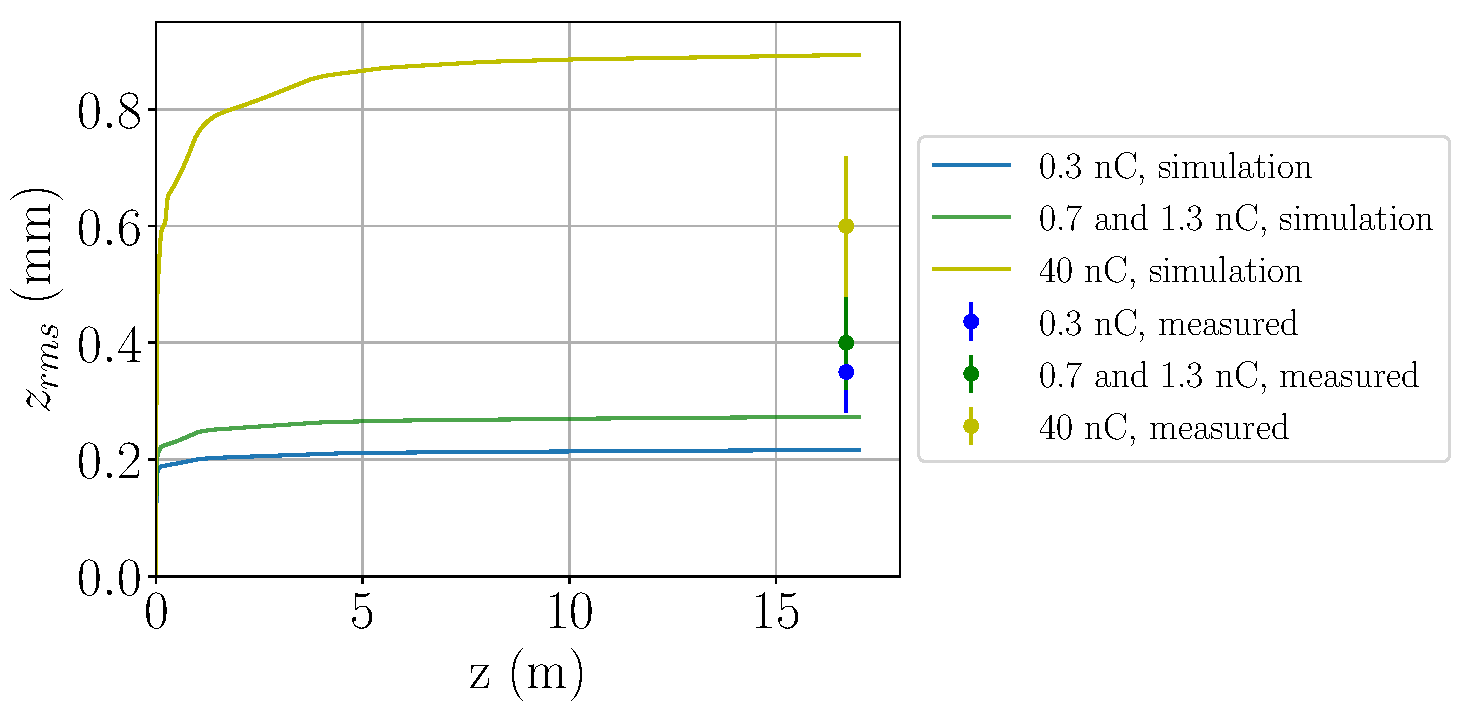
\includegraphics[width=0.75\linewidth]{images/THPMF048f5}
	\caption{Comparison of simulations and experimental measurements.}
	\label{sims}
\end{figure*}
While there is not an exact match, the results follow the same trends.
The discrepancies indicate there are still adjustments that can be made
to the simulation model. Since the bunch length does not change measurably 
after the gun, it is reasonable to suspect one of the parameters in the 
gun is the source of the discrepancy. Gun simulation parameters include the laser radius, 
solenoid strengths, gradient, and emission model. The solenoid strength is ruled 
out due to the recent measurement discussed in Chapter~\ref{chp:exp}. 
Laser radius discrepancies should only impact the transverse beam dimensions 
through coupling of the space charge force which is accounted for the in simulation. 
Also, it is now known that the gun gradient is lower than expected.
One other source of error could be the longitudinal laser profile.
There is currently no way to measure this at the AWA. 

Agreement is likely to improve as more of these measurements are made. 
These can include better measurements of the beam energy and careful attention to other 
beam line parameters such as the laser radius and solenoid strengths.
In the case of high charge simulations, where the agreement is the worst, 
more consideration is needed for large charge fluctuations in the data.
When running at high charge the fluctuations in the laser intensity can results in 
large swings in the bunch charge (i.e. \SI{20}{nC} to \SI{40}{nC}. 
In attempts to compensate for this, large amounts of data were taken and some 
outliers removed. Perhaps a more through analysis of the charge distribution is needed. 

Experimentally measured values of the bunch duration and bunch length are shown in Table~\ref{exp}.
Note the bunch length is shown in Figure~\ref{sims}. 
The table gives bunch duration, and the plot gives bunch length for the same data.
\begin{table}[h]
	\centering
	\caption{Experimental Bunch Length Measurements}
	\rowcolors{2}{blue!15}{white}
	\begin{tabular}{rccc}
		\toprule
		\toprule
		\textbf{Charge} & \thead{\textbf{Bunch Dur.}\\ \textbf{(RMS)}} & \thead{\textbf{Bunch Length}\\\textbf{(RMS)}} & \textbf{Laser spot size}  \\
		\midrule
		\SI{0.3}{nC} & \SI{2.2}{ps} &  \SI{0.33}{mm} & 4 mm    \\ %[3pt]
		\SI{0.7}{nC} & \SI{2.6}{ps} &  \SI{0.36}{mm} & 4 mm   \\ %[3pt]
		\SI{1.3}{nC} & \SI{2.6}{ps} &  \SI{0.39}{mm} & 4 mm    \\
		\SI{30}{nC}  & \SI{4.1}{ps} &  \SI{0.615}{mm} & 9 mm \\ %[3pt]
		\bottomrule
	\end{tabular}
	\label{exp}
\end{table}

%%%%%%%%%%%%%%%%%%%%%%%%%%%%%%%%%%%%%%%%%%%%%%%%%%%%%%%%%%%%%%%%%%%%%%%%%%%%%%%%
%%%%%%%%%%%%%%%%%%%%%%%%%%%%%%%%%%%%%%%%%%%%%%%%%%%%%%%%%%%%%%%%%%%%%%%%%%%%%%%%
\Section{Optimization} \label{sec:opt}

Throughout the design process, optimization algorithms 
were used to study the beam parameters at the entrance of the TBA experimental area.
Minimizing the emittance and bunch length after the six cavity linac,
and choosing the optimal optics configuration for maximum beam transport 
were the main objectives of all optimization work.
The techniques used include model-based, genetic,
and structure exploiting algorithms. 
 
Model-based, derivative-free, trust-region algorithms 
are increasingly popular in mathematics for optimizing computationally 
expensive numerical simulations. The term model-based means 
that the simulation output is used to construct a model. 
This can be a quadratic function as described later, 
or something more complex.
Derivative-free optimization indicates there is no one 
governing equation that defines all simulation output
for a given set of inputs. For example, there is no 
function for beam size that allows calculation of a derivative. 
Many common optimization techniques calculate derivatives, 
but this is not applicable in situations of complex dynamics.
Finally, trust-region refers to the bounds on our input variables.
There are physical constraints on the magnet and RF values that 
can be achieved in the real world. This information is used 
to bound the optimization work in a ``trust-region'', so that
effort is not wasted in an infeasible search space.
A strength of model-based methods is their efficient use of function evaluations. 

After a model-based method was implemented, 
a common optimization technique was used to benchmark the results. 
The algorithm used for confirmation 
is called a genetic algorithm (GA). An implementation of this algorithm is
built into \verb|OPAL|. GA's follow nature's lead as the name suggests.
A random sample is done, and the best points based on the defined objectives
(i.e. emittance, bunch length, beam size, etc.)
are selected. Those points are then mixed to form a new ``generation''
and a new round of simulations is started. This method continues
until some convergence criteria are met. While this method does 
produce results, and is widely used, it requires large amounts 
of computational resources to to reach convergence.
This is the most commonly used optimization in accelerator physics
at the moment. Preliminary designs 
for the TBA optics configuration were probed using the GA in \verb|OPAL|. 



\Subsection{Model Based Methods}
%\section{Optimization Algorithm}
% ----------------------------------------------------
The model-based algorithm was the first type of algorithm used to optimized the beam dynamics 
in two cases of interest at the AWA.
The first case was for lower beam charge, and used only the gun parameters for the optimization.  
The second case was for higher beam charge, and included parameters of the downstream linac as well as the gun.
In the first case,  the emittance of a \SI{1}{nC} electron 
bunch produced by the AWA RF photocathode gun 
was minimized by adjusting three parameters: RF gun phase, 
solenoid strength, and laser radius. The algorithm 
converged to a set of parameters that yielded an
emittance of \SI{1.08}{\um}. In the second case, 
the number of optimization parameters was expanded to model the complete AWA RF 
photoinjector (the gun and six accelerating cavities) at \SI{40}{nC}. 
The optimization algorithm was used in a Pareto study; which is a type of study that compares the 
trade-off between competing parameters, such as emittance and bunch 
length at the exit of the AWA \SI{70}{MeV} photoinjector. 

Model-based, derivative-free algorithms are frequently used to optimize
computationally expensive simulations due to their judicious use of function
evaluations. In cases specific to accelerator physics, 
beam properties at different operational parameters are observed;
these methods then build models of the unknown
function and minimize these models to identify candidate parameters to 
evaluate. Bounded Optimization BY Quadratic Approximation (BOBYQA)~\cite{bobyqa},
 is one such method that is available via the
NLopt~\cite{nlopt} package and was used in this study. 
Given a candidate set of optimal parameters $v^k$, BOBYQA
constructs a quadratic model using function values of points near $v^k$. 
This model is minimized in a neighborhood of $v^k$ in order to produce a point $\hat{v}$. 
If $\hat{v}$ has a smaller objective function value than $v^k$, 
the estimate of the optimum is updated to $\hat{v}$, and a new model is constructed. 
If $\hat{v}$ is not a sufficient improvement over $v^k$, 
the model around $v^k$ is improved. For more
information about derivative-free optimization, see~\cite{Conn2009a}.

The parameters $v^k$ are generated and supplied to \verb|OPAL-t|~\cite{opal}. 
The optimization package NLopt and \verb|OPAL-t| were used
in combination with Python code written at ANL with the help 
of Jeffrey Larson, to perform simulation evaluations and optimization.
All the files needed to replicate the results in this section are available at: 
\url{<$www.mcs.anl.gov/$\sim$jlarson/AWA$>}.  

\Subsection{Optimization Parameters}
% ----------------------------------------------------
When optimizing the gun, three parameters $v^k$ were varied: 
solenoid strength ($S_3$), gun phase ($\phi_g$), 
and laser radius ($R$) of a uniform photon distribution. 
The minimized objective was emittance ($\epsilon_x$).
(The reference phase of the gun is defined as $0^{\circ}$ at maximum accelerating voltage.) 
When optimizing the gun and the entire linac, seven additional parameters were 
varied: the longitudinal duration of the laser pulse, defined at full width at half maximum ($T$)
and accelerating cavity phases ($\phi_L$). The optimization parameters and
bounds are given in Table~\ref{tab:parameters}; the set of
ten optimization parameters are denoted as $v=[S_3, \phi_g, R, T, \phi_L]$, where 
$\phi_L=[\phi_{L_1},\ldots,\phi_{L_6}]$ represents the phase of each linac cavity $L_1$-$L_6$. 
\begin{table}
	\caption{\label{tab:parameters} Parameter bounds for gun and linac optimization.}
	\begin{center}
		\begin{tabular}{ l *{3}{c}} 
			\toprule
			\textbf{Variable} & \textbf{Range} & \textbf{Unit} \\
			\midrule
			Solenoid Strength & $ 0 \le S_3 \le 440$  & amps \\
			Phase of Gun & $-60 \le \phi_g \le 60$  & degrees \\
			Laser Radius  & $0.1 \le R \le 30$  & mm \\
			Laser FWHM & $2 \le T \le $10  & ps \\
			Cavity Phase  & $-20 \le \phi_L \le 20$  & degrees \\
			\bottomrule	
		\end{tabular}
	\end{center}
\end{table}


\Subsection{Gun Simulations Using BOBYQA} \label{sec:gunbobyqa}
%\section{Gun Optimization}
% ----------------------------------------------------
There has been work done by other groups to optimize 1.5-cell RF guns
at \SI{1}{nC}~\cite{pitz}. The known solution from that work was used as 
a baseline test of BOBYQA when applied to this accelerator application.
An optimization of the single objective emittance ($\epsilon_x$) was 
performed over a length of \SI{5}{m}. 
All linacs were turned off and only gun parameters were varied. 
Non-varying parameters are listed in Table~\ref{tab:gun}; 
their values are based on realistic parameters at PITZ and AWA~\cite{pitz, benchmark}.

Local optimization runs were started using five points 
with different design variables. All optimization runs converged 
(in less than 100 function evaluations) to a parameter set ($S_3=\SI{269}{A}$,
$\phi_g=\SI{-3.0}{^{\circ}}$, and $R=\SI{0.6}{mm}$) with an emittance of $\SI{1.08}{\um}$.
An exhaustive search of the parameter space was not done, and there may be other local minima that were not found.
However, the results match expectations based on the literature. 
\begin{table}%[h] 
	\caption{\label{tab:gun} Non-varying parameters for gun optimization.}
	\begin{center}
		\begin{tabular}{lll}
			\toprule
			\textbf{Parameter} & \textbf{Value} \\
			\midrule
			Charge  & \SI{1}{nC} \\
			Gradient & \SI{60}{MV/m} \\
			Laser FWHM & \SI{20}{ps} \\
			Laser Rise and Fall Time & \SI{6}{ps} \\
			Kinetic Energy at Cathode  & \SI{0.55}{eV} \\
			$S_1$ and $S_2$ & \SI{550}{A} \\
			\bottomrule
		\end{tabular}
	\end{center}
\end{table}

\Subsection{Linac Optimization}\label{sec:linacopt}
Next a multiobjective optimization of the linac (Figure~\ref{fig:beamline}) was done, 
by adjusting the ten parameters in Table~\ref{tab:parameters}. The charge was set to \SI{40}{nC}
and was chosen to match upcoming two-beam acceleration experiments~\cite{tba2017}. 
Two objectives were considered: emittance and bunch length ($\sigma_z$). 
The location of interest is $z_1=\SI{12.51}{m}$, as this is the entrance of the first 
quadrupole magnet after the linac. Optimization was required only for the horizontal emittance, $\epsilon_{x}$.  
This is because there were no asymmetric focusing elements in the linac, and the beam is round, $\epsilon_{x}=\epsilon_{y}$. 
The non-varying parameters for all linac simulation runs are shown in Table~\ref{tab:linac}. 
These are typical operating conditions at AWA. 
The particle distribution initially emitted from the cathode is generated within \verb|OPAL-t| 
using input parameters such as the cathode material, the work function and the laser energy.  

\def \gunleft {-1.0}
\def \gunright {0.3}
\def \loneright {1.0}
\def \ltworight {3.5}
\def \lthreeright {5.0}
\def \lfourright {7.0}
\def \lfiveright {8.5}
\def \lsixright {10}
\begin{figure*}
	\begin{center}
		
		\begin{tikzpicture}[scale=0.95]
		%Gun drawings
		\draw[fill=orange, very thick, rounded corners =0.1cm] (\gunleft,0.5)rectangle (\gunright,1.5) node[pos=.5, white] {\textbf{Gun}} ;
		
		%S1
		\node[] at (-1.3,2.9) {$S_1$};
		\draw[ultra thick, fill=black!60!green] (-1.4,-0.5)rectangle  (-1.0,0.5) node[pos=.5, white] {} ;
		\draw[black, ultra thick] (-1.4,-0.5) -- (-1.0,0.5);
		\draw[black, ultra thick] (-1.4,0.5) -- (-1.0,-0.5);
		\draw[ultra thick, fill=black!60!green] (-1.4,1.5)rectangle  (-1.0,2.5) node[pos=.5, white] {} ;
		\draw[black, ultra thick] (-1.4,1.5) -- (-1.0,2.5);
		\draw[black, ultra thick] (-1.4,2.5) -- (-1.0,1.5);
		%S2
		\node[] at (-0.8,2.9) {$S_2$};
		\draw[ultra thick, fill=black!60!green] (-1.0,-0.5)rectangle  (-0.6,0.5) node[pos=.5, white] {} ;
		\draw[black, ultra thick] (-1.0,-0.5) -- (-0.6,0.5);
		\draw[black, ultra thick] (-1.0,0.5) -- (-0.6,-0.5);
		\draw[ultra thick, fill=black!60!green] (-1.0,1.5)rectangle  (-0.6,2.5) node[pos=.5, white] {} ;
		\draw[black, ultra thick] (-1.0,1.5) -- (-0.6,2.5);
		\draw[black, ultra thick] (-1.0,2.5) -- (-0.6,1.5);
		
		%S3
		\node[] at (0.2,2.9) {$S_3$};
		\draw[ultra thick, fill=black!60!green] (-0.1,-0.5) rectangle  (0.3,0.5) node[pos=.5, white] {};
		\draw[black, ultra thick] (-0.1,-0.5) -- (0.3,0.5);
		\draw[black, ultra thick] (-0.1,0.5) -- (0.3,-0.5);
		\draw[ultra thick, fill=black!60!green] (-0.1,1.5) rectangle  (0.3,2.5) node[pos=.5, white] {};
		\draw[black, ultra thick] (-0.1,1.5) -- (0.3,2.5);
		\draw[black, ultra thick] (-0.1,2.5) -- (0.3,1.5);
		%Linac drawings 
		\draw[fill=blue, ultra thick, rounded corners =0.1cm] (\loneright,0)rectangle  ({\loneright+0.84},2) node[pos=.5, white] {$L_1$} ;
		\draw[fill=blue, ultra thick, rounded corners =0.1cm] (\ltworight,0)rectangle  ({\ltworight+0.84},2) node[pos=.5, white] {$L_2$};
		\draw[fill=blue, ultra thick, rounded corners =0.1cm] (\lthreeright,0)rectangle ({\lthreeright+0.84},2) node[pos=.5, white] {$L_3$};
		\draw[fill=blue, ultra thick, rounded corners =0.1cm] (\lfourright,0)rectangle ({\lfourright+0.84},2) node[pos=.5, white] {$L_4$};
		\draw[fill=blue, ultra thick, rounded corners =0.1cm] (\lfiveright,0)rectangle ({\lfiveright+0.84},2) node[pos=.5, white] {$L_5$};
		\draw[fill=blue, ultra thick, rounded corners =0.1cm] (\lsixright,0)rectangle ({\lsixright+0.84},2) node[pos=.5, white] {$L_6$};
		\draw[very thick] (\gunleft,-1.5) -- (14,-1.5);
		\draw[latex-latex] (\gunleft,-1.5) -- (14,-1.5) ; 
		\foreach \x in  {0.3, 1.0, 3.5, 5.0, 7.0, 8.5, 10, 12.5} %tick marks
		\draw[shift={(\x,-1.5)},color=black] (0pt,3pt) -- (0pt,-3pt);
		\foreach \x in {0.3, 1.0, 3.5, 5.0, 7.0, 8.5, 10, 12.5}
		\draw[shift={(\x,-1.7)},color=black] (0pt,0pt) node[below] 
		{$\x$};
		
		\node[draw, fill=yellow, star, star points=5, star point ratio=0.6, minimum size=0.6cm]
		at (12.5,1.0) {$z_1$};
		\end{tikzpicture}
	\end{center}
	\caption{Layout of the AWA linac. The \SI{70}{MeV} AWA RF photoinjector 
		is an RF gun followed by a linac with six RF accelerating cavities, 
		labeled $L_1$-$L_6$ \cite{Power:2010zza}.  The cavity phases are controlled independently. 
		The 1.5-cell RF gun operates at \SI{1.3}{GHz} with three solenoids 
		and a Cs$_{2}$Te photocathode excited by a \SI{248}{nm} UV laser.  
		Solenoid 1 ($S_1$) is used to buck the field at the cathode,
		while the other two solenoids ($S_2$ and $S_3$) are used for emittance compensation.  
		Tick marks are located at the exit of the gun, entrance of
		each accelerating cavity, and location of optimization.}
	\label{fig:beamline} 
\end{figure*} 
\begin{table}%[h] %or [hbt] ?
	\caption{\label{tab:linac} Non-varying parameters for linac optimization.}
	\begin{center}
		\begin{tabular}{lll}
			\toprule
			\toprule
			\textbf{Parameter} & \textbf{Value} \\
			\midrule
			Charge  & \SI{40}{nC} \\
			Laser Rise and Fall Time & \SI{1.0}{ps} \\
			Gun Gradient & \SI{70}{MV/m} \\
			$S_1$ and $S_2$ & \SI{550}{A}\\
			Cavity Gradient $L_1$--$L_4$ & \SI{25}{MV/m} \\
			Cavity Gradient $L_5$--$L_6$ & \SI{27}{MV/m} \\
			\bottomrule
		\end{tabular}
	\end{center}
\end{table}

A 1,000 point sample of linac parameters were drawn from the domain
in Table~\ref{tab:parameters} and simulated. Of these, 132 simulations completed
without error, and the emittance and bunch length at $z_1=\SI{12.51}{m}$ was
recorded for each of these points. From the sample of the 132 successful simulations 
the minimum and maximum values of emittance and bunch length
were found (i.e: $\epsilon_{\min}$ and $\epsilon_{\max}$). 
The raw $\epsilon_x(v,z_1)$ and $\sigma_z(v,z_1)$ sample values were then
shifted and scaled to produce $\bar{\epsilon}_x(v,z_1)$, and $\bar{\sigma}_z(v,z_1)$,
which have a minimum value of 0 and a maximum value of 1 over the 132-point sample set. That is, 
\begin{equation}
\bar{\epsilon}_x (v,z_1) = \frac{ \epsilon_x (v,z_1) - \epsilon_{\min} } { \epsilon_{\max} - \epsilon_{\min} }\, ,
\label{eq:scale}
\end{equation} 
and $\bar{\sigma}_z (v,z_1)$ is defined similarly.
This scaling is done in order to remove the difference in the units between
emittance and bunch length when optimizing.

With the scaled values of $\bar{\epsilon}_x$ and $\bar{\sigma}_z$, a sequence
of eleven optimization problems were solved by minimizing,
\begin{equation}
f(v,w) = w \,\bar{\epsilon}_x(v,z_1) + (1-w)\, \bar{\sigma}_z(v,z_1)\, ,
\label{eq:newobj}
\end{equation}
for $w \in \left\{ 0, 0.1, \ldots, 1 \right\}$. 
For each weight $w$, BOBYQA was started from the sample point with the 
smallest value of $f(v,w)$.  From the initial random sample, six unique starting points were chosen. 
(There were fewer starting points than weights because some samples had the smallest objective value for multiple weights. 
For example, the smallest values of $f(v,0.4)$, $f(v,0.5)$, and $f(v,0.6)$ occurred when at the eighteenth sample point.)
Some $f(v,w)$ values also had one or more linac phases near the initial $\pm20^{\circ}$ boundary. 
The $\phi_L$ boundary was expanded to $\pm40^{\circ}$ for those BOBYQA runs.

\Subsection{Pareto Front for AWA Linac}
%\section{Pareto Front for AWA Linac} 
% ----------------------------------------------------
Since multiple objectives are under consideration in this case, a
trade-off analysis is necessary. 
\begin{figure}%[h]
	\begin{center}
		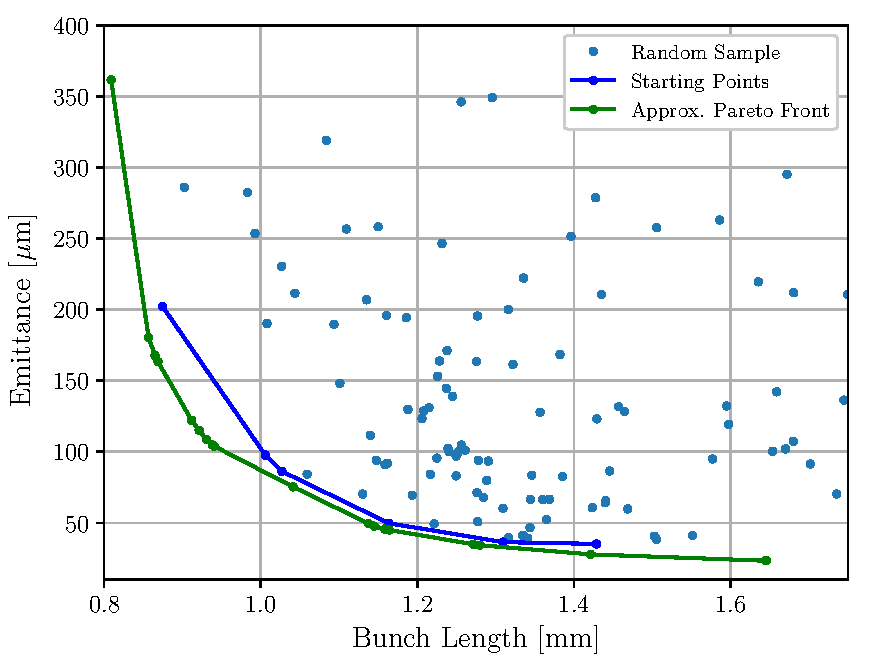
\includegraphics[width=0.75\textwidth]{images/THPAB155f1}
		\caption{Random sample results, starting sample points, and resulting approximate Pareto front for the linac at \SI{40}{nC}. The Pareto front is the result of all BOBYQA evaluations.}
		\label{fig:pareto}
	\end{center}
\end{figure}
This can be aided by examining a Pareto front: the set of parameters 
for which no other point exists that is better with respect to both objectives~\cite{ehrgott2006multicriteria}.
In Figure~\ref{fig:pareto}, blue dots show the emittance and bunch length for the
evaluated random sample. The sample points for which no other point has better
emittance and bunch length are connected with a blue line. BOBYQA was started
from these points, as described above, producing the green approximate Pareto front. 

The number of simulation evaluations needed to obtain convergence
in the BOBYQA runs varied from a minimum of 107 evaluations to a maximum of 208 
evaluations. In order to generate the Pareto front in
Figure~\ref{fig:pareto}, a total of 2,492 simulation evaluations were completed.
Most simulation evaluations took approximately 7 minutes, using 16 cores and 100,000 particles. 
These numbers are driven by the amount of time \verb|OPAL-t| needs to simulate the beam line. 

The best-found objective value through each BOBYQA run is shown in Figure~\ref{fig:iterations}. 
Weight 0.0 and 1.0 are negative due to the scaling in Equation~(\ref{eq:scale}). While the weights, $w$, are always non-negative, 
$\bar{\epsilon}_x (v,z_1)$ or $\bar{\sigma}_z(v,z_1)$ will be negative if BOBYQA finds a point with a value of 
$\epsilon_x(v,z_1)$ or $\sigma_z(v,z_1)$ that is less than $\epsilon_{\min}$ or $\sigma_{\min}$ from the initial sample. 
\begin{figure}%[h]
	\begin{center}
		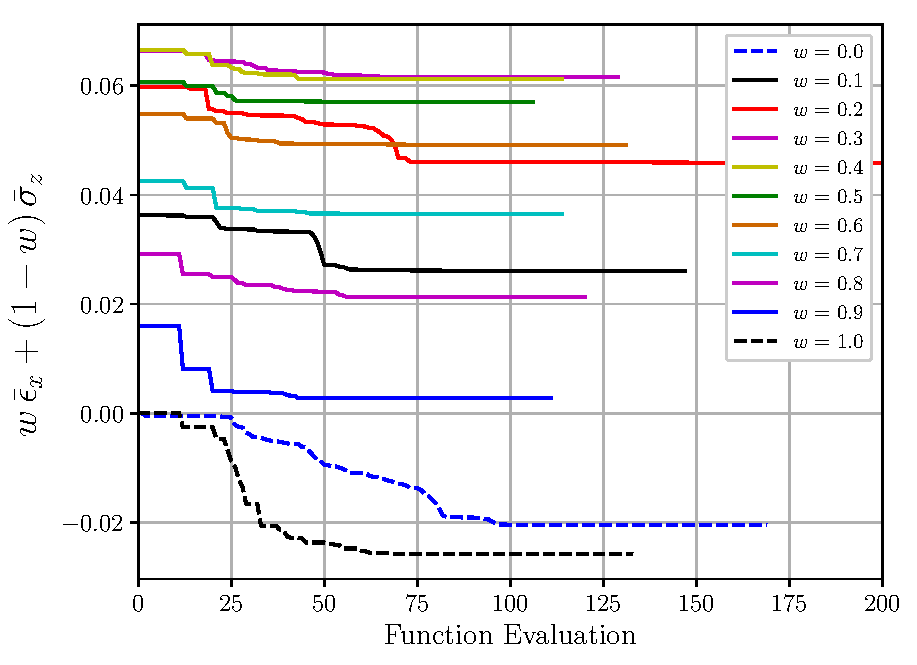
\includegraphics[width=0.75\textwidth]{images/THPAB155f2}
		\caption{\label{fig:iterations}Eleven optimization runs were started, one corresponding to each weight in Eq.~\ref{eq:newobj}.
			Each time a simulation was completed, the objective function, $f$, was evaluated and the next simulation inputs were 
			decided by BOBYQA. The minimum observed objective function values are plotted for the runs at \SI{40}{nC}.
			When the objective function converged to $10^{-4}$, the optimization runs were stopped. 
		}
	\end{center}
\end{figure}

Note that seven of the BOBYQA runs converged to emittance values
between \SI{20}{\mu m} and \SI{50}{\mu m}, which is shown in Figure~\ref{fig:trade} 
along with gun phase and bunch length for each of the 11
optimized points. Figure~\ref{fig:trade} is annotated with $T$ because that parameter 
shows strong correlation with the gun phase. Other optimized parameters such as the laser radius were found to stay within a 
narrow range (\SIrange{10}{16}{mm}).  
\begin{figure}%[h]
	\begin{center}
		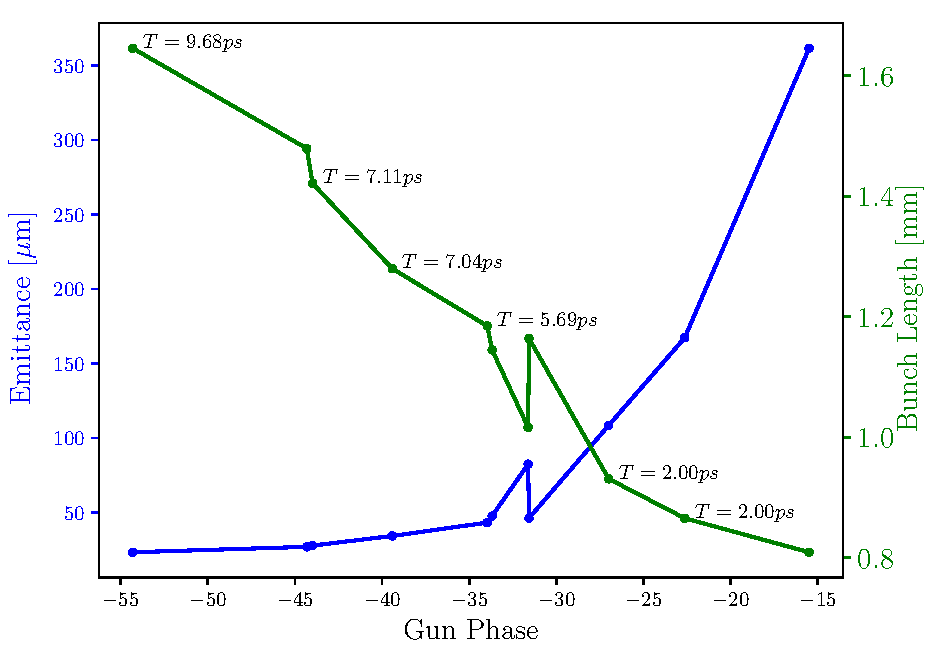
\includegraphics[width=0.75\textwidth]{images/THPAB155f3}
		\caption{\label{fig:trade}Bunch length and emittance vs.~gun phase at each optimized point in the Pareto front for the linac at \SI{40}{nC}. The phase of the max energy gain is $0^{\circ}$.}
	\end{center}
\end{figure}


The optimized linac phases maximize energy gain while minimizing the energy spread.
The energy spread of the beam exiting the gun depends strongly on $\phi_g$.
There are three distinct regions where the optimized points had similar gun phases 
(less than $\pm10^{\circ}$) which resulted in nearly identical linac phases. For example:  
all six phases, $\phi_L$, varied by less than $10^{\circ}$ for $w \in \left\{ 0, 0.1\right\}$,
less than $5^{\circ}$ for $w \in \left\{ 0.4, 0.5, 0.6\right\}$, 
and less than $10^{\circ}$ for $w \in \left\{ 0.7, 0.8, 0.9\right\}$.
This indicates optimized linac phases may benefit a range of gun settings during operation. 


\Subsection{Lessons Learned from BOBYQA Work}
Using an AWA beam line as the simulation model, the BOBYQA algorithm was used 
to optimize the emittance produced by the gun at \SI{1}{nC}.
Using the same algorithm, a multiobjective analysis for the linac at \SI{40}{nC}, was performed. 
A Pareto front comparing the trade-off between bunch length and emittance was generated for the linac. 
In total, only 2,492 simulation evaluations were needed to produce the approximate Pareto front.
From this work a few key take aways are clear. First, larger laser radius
is uniformly better for high charge. i.e large radius helps lower emittance.
The second clear results is alternating the phases in the linac can control 
the energy spread created by the gun, i.e. running off crest in the linac 
can reduce the energy spread significantly.

%%%%%%%%%%%%%%%%%%%%%%%%%%%%%%%%%%%%%%%%%%%%%%%%%%%%%%%%%%%%%%%%%%%%%%%%%%%%%%%%
%%%%%%%%%%%%%%%%%%%%%%%%%%%%%%%%%%%%%%%%%%%%%%%%%%%%%%%%%%%%%%%%%%%%%%%%%%%%%%%%
\Subsection{Genetic Algorithm: NSGA-II} \label{sec:ga}
%%%%%%%%%%%%%%%%%%%%%%%%%%%%%%%%%%%%%%%%%%%%%%%%%%%%%%%%%%%%%%%%%%%%%%%%%%%%%%%%
%%%%%%%%%%%%%%%%%%%%%%%%%%%%%%%%%%%%%%%%%%%%%%%%%%%%%%%%%%%%%%%%%%%%%%%%%%%%%%%%
While the model-based results are promising, 
GA's are the most commonly used type of optimization algorithm in the accelerator community.
In particular the Non-dominated Sorting Genetic Algorithm II (NSGA-II)~\cite{NSGA}, 
is the implementation that is most commonly used.
To validate that the model-based method was giving comparable results to what a GA would give, 
a low fidelity version of the linac simulation in Section~\ref{sec:linacopt} was formulated.
This fidelity change included reducing the number of particles and grid points. 
The boundaries on the design variables were also reduced to ensure only 
feasible simulation points were evaluated.

Figure~\ref{fig:GAvsModel} clearly shows the optimized simulations results from 
the GA and model-based method are similar. Both methods gave desirable 
results for the linac optimization problem. 
The main difference between the two methods is the amount of computational 
resources needed, see the comparison in Table~\ref{tab:optcompare}.
Note, that as a general rule of thumb, most people simulate at least 100 generations, before stopping a GA.
This suggests that while the model-based method and GA will arrive at 
the same conclusion, there may be a difference in computation resources required. 
The time to solution for the two cases can be significantly different, 
order thousands of compute hours.
\begin{figure}
	\centering
	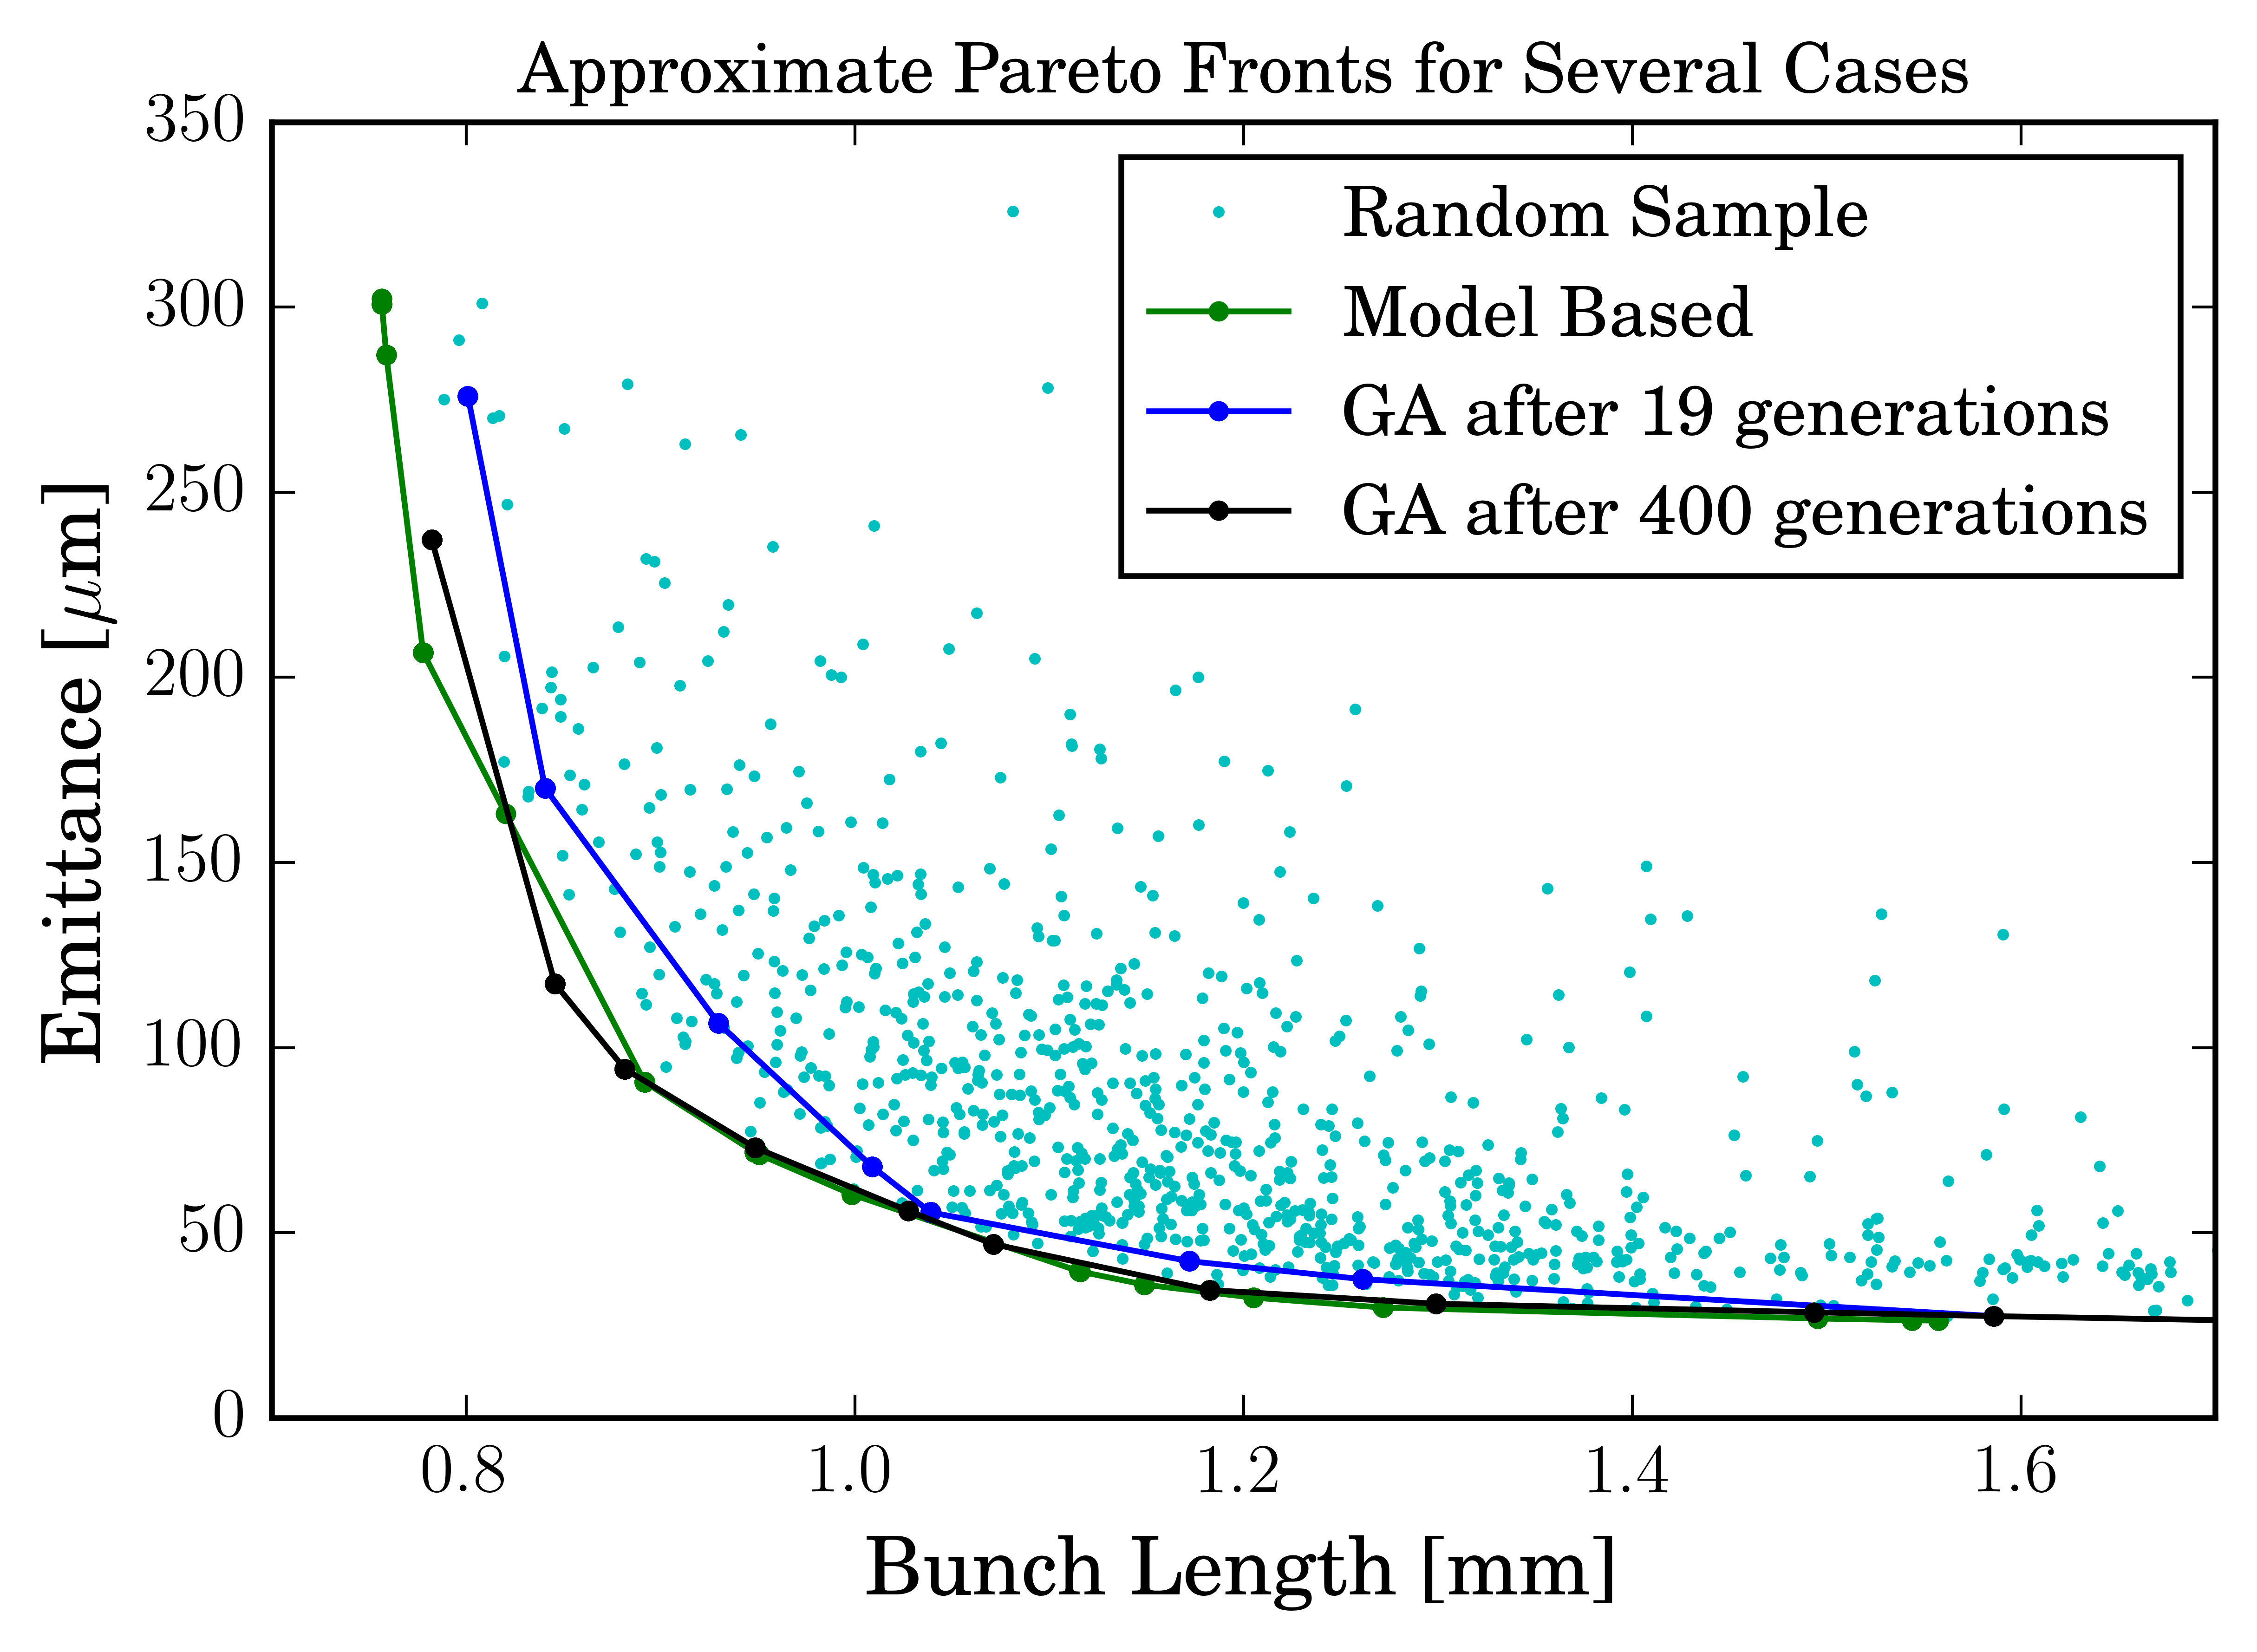
\includegraphics[width=0.75\textwidth]{./images/model_vs_ga}
	\caption{Comparison of model-based and GA simulations results.}
	\label{fig:GAvsModel}
\end{figure}
\begin{table}%[h] %or [hbt] ?
	\caption{Number of simulation evaluations for model-based and GA optimizations.
	These numbers correspond to the lines in Figure~\ref{fig:GAvsModel}.}
	\label{tab:optcompare}
	\begin{center}
		\begin{tabular}{lcc}
			\toprule
			\toprule
			\textbf{Optimization} & \textbf{Number of Simulations} & \textbf{Compute Hours} \\
			\midrule
			Model Based  		& 2393  & 79.8 \\
			GA 19 Generations 	& 2432  & 81.1 \\
			GA 200 Generations 	& 25600 & 853.3\\
			GA 400 Generations 	& 51200 & 1706.7\\
			\bottomrule
		\end{tabular}
	\end{center}
\end{table}

\Section{Chapter Summary}

PIC simulations of the AWA drive line are essential to the TBA project. 
Accurate predictions of the beam dynamics in the drive line are needed for the 
success of fully staged TBA, especially with the tighter tolerances required by the PETS apertures.
A new code, \verb|OPAL-t|, was investigated as an alternative to \verb|ASTRA| and \verb|GPT|. 
The benefits of \verb|OPAL| include being free and being able to run on a parallel platform.
A benchmark was done to ensure that \verb|OPAL| gave results consistent with other codes used by members of the AWA.
No major discrepancies were found in the space charge and CSR algorithms.
Although, note that the \verb|OPAL| CSR routine can not be used for low energy beams.
Convergence studies were also done to determine base line computational 
parameters for future simulations.
After benchmarking, all PIC simulations of the TBA beam line were performed using \verb|OPAL-t| on clusters provided by ANL.

Next, optimization to find a set of operating parameters for
\SI{40}{nC} TBA experiments was done. A model-based method BOBYQA was used to optimize the gun and linac. 
From these results it is clear that the laser radius should be as large as possible to mitigate space charge forces.
In addition, the RF cavities should be run off crest to minimize energy spread.
Validation of the model-based method was done by doing a comparison with the commonly used GA method. 
The results agreed well, and suggest that the model-based methods require fewer computational resources than a GA. 

Validation of \verb|OPAL-t| and initial optimization studies provided a tool 
to design the beam transport to the TBA experimental area.  
Initial probes into this problem were done using the genetic algorithm
implemented in \verb|OPAL-t|~\cite{optpilot}. Details of this work can be found in Chapter~\ref{chp:4}.





